\chapter{背景与相关工作}
\label{chap:background}

本章将详细介绍静态时序分析（Static Timing Analysis, STA）与公共路径悲观消除（Common Path Pessimism Removal, CPPR）的理论基础。首先，回顾数字集成电路中时序验证的基本概念，包括基于图论的延时模型计算以及当前工业界广泛采用的快速-慢速时序模型（Early-Late Timing Model，或称片上变异 OCV 模型）。其次，深入剖析由 OCV 模型所引发的公共路径悲观现象，并给出 CPPR 修正的核心计算原理。在此基础上，系统梳理并分类探讨目前用于处理带有 CPPR 的大规模网络分析的两大主流流派：“先消除后搜索（CPPR-before-search）”与“搜索与悲观消除并进（CPPR-during/after-search）”。最后，本章将详细对比并分析现有算法在面对现代千万门级超大规模集成电路验证时所遇到的一系列由于图重汇聚与组合爆炸导致的极高计算复杂度以及扩展性瓶颈问题，从而自然地引出本课题所提出的研究动机与解决方案框架。

\section{静态时序分析与片上变异模型基础}
\label{sec:sta_basics}

静态时序分析是数字芯片设计签核（Sign-off）流程中最为重要和最耗时的步骤之一。在现代EDA工具中，一个数字电路网表通常会被建模为一个带有延时的有向无环图（Directed Acyclic Graph, DAG），称为时序图（Timing Graph）。

\subsection{时序图模型与基本概念}
对于一个典型的时序图 $G = (V, E)$，顶点集 $V$ 代表了电路中的各个电气节点，主要包括逻辑门的输入/输出引脚（Pin）、主时钟源节点、以及各类寄存器的时钟引脚和数据引脚等。边集 $E$ 则表示引脚之间的信号传播路径。边在物理上可能对应于逻辑门内部的信号传播（Cell Delay）或不同逻辑器件互连线上的传输延迟（Net Delay）。

在时序图上，最为核心的计算涉及两个概念：到达时间（Arrival Time, AT）与要求时间（Required Time, RT）。
\begin{itemize}
    \item \textbf{到达时间 (AT)}：指信号自源节点产生并经过前序电路网络传播至当前关注节点 $v$ 处所需的最短或最长时间。
    \item \textbf{要求时间 (RT)}：指为保证电路在指定时钟频率下正确工作以及遵循设定的设计约束（如建立时间和保持时间），信号必须在何时之前（或之后）到达节点 $v$。
\end{itemize}

结合这两者的计算，时序分析通过计算\textbf{时序裕度（Slack）}来直观地评估当前节点上的时序是否安全：
\begin{equation}
    Slack(v) = RT(v) - AT(v)
\end{equation}
若 $Slack \geq 0$，则表示该节点满足时序要求；反之，若 $Slack < 0$，则说明发生了时序违例（Timing Violation），存在导致系统功能失效的致命风险。设计者在优化时，总是优先寻找 $Slack$ 最低（即负向最大值）的时序路径，这些路径被称为关键路径（Critical Path）。

\subsection{快速-慢速时序模型 (OCV)}
传统的 STA 往往假设电路元件的工作条件是固定且均匀的。然而，在纳米级甚至先进的 FinFET 工艺中，同一块晶圆上的不同区域，或同一芯片上的不同门电路，由于制造工艺偏差（Process）、工作电压波动（Voltage）、以及局部温度分布不匀（Temperature）等因素的复合影响交织，其信号传播延迟并不是一个确定值。

为刻画这种不确定性，工业界极其依赖于由上述 PVT 变量综合推导而来的快速-慢速时序模型（Early-Late Timing Model，常称为 OCV模型）\cite{TODO_ocv_model}。OCV 为时序图中所有节点和连线的时延定义了两个极端边界：
\begin{itemize}
    \item $d_{early}(e)$：元件/连线在最理想、最快工作环境下的最短极值传播时延。
    \item $d_{late}(e)$：元件/连线在最恶劣、最慢工作环境下的最长极值传播时延。
\end{itemize}
在执行安全评估（Soundness Proof）时，如果要计算最悲观情况下的建立时间（Setup Time）裕度，分析器会假设数据（Data）传播路径处在极其缓慢的 $d_{late}$ 状态，而试图捕获该数据的时钟信号（Clock）经历极度顺畅的 $d_{early}$ 状态，反之亦然。这种通过构造最差运行组合来掩盖所有理论波动的办法，极大地提高了签核结果的可靠性。

\section{公共路径悲观现象与CPPR原理}
\label{sec:cppr_theory}

虽然 OCV 快速-慢速模型能够在静态检查中包容随机物理波动，从而为芯片产品提供强有力的时序安全底线，但其由于极端的包络假设也引入了严重的数学悖论：即公共路径悲观（Common Path Pessimism, CPP）。

\subsection{悲观现象的物理背景}
在同步数字电路中，由同一个时钟源（Clock Root）发出的时钟信号，往往在经过一段共同的缓冲器网络（Buffer Tree）后才会产生分叉，分别传播向两个相互连接的触发器——源触发器（Launch Flip-Flop）和目的触发器（Capture Flip-Flop）。在计算前文所述的最严苛 Setup 时序松弛量时，根据 OCV 规则，EDA 工具需要对到达源触发器的时钟路径采用慢速延迟（$d_{late}$），从而让发射变晚；而对到达目标触发器的时钟路径则采用快速延迟（$d_{early}$），让捕获窗口尽量前移。

\begin{figure}[htbp]
  \centering
  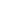
\includegraphics[width=0.8\linewidth]{images/cppr_clock_tree_example.png}
  \caption{TODO：需要一张时钟树展示公共节点分离成早晚路径导致悲观现象的示意图。图应清晰标出 Launch Path, Capture Path, 以及汇聚前的共同缓冲器节点（Common Node）。}
  \label{fig:cppr_clock_tree}
\end{figure}

然而，在时钟发生分叉前的这段“公共路径”（Common Path，如图~\ref{fig:cppr_clock_tree} 所示）上，既同时属于发射分支，又归属捕获分支。这就意味着分析器硬生生地将同一个物理缓冲器在\textbf{绝对相同的时刻}假想为既处在“极慢”的极端工艺/温度环境，同时又处于“极快”的优异工作环境中。由于一个物理实体在某一瞬间不可能体现为截然相反的两种性能，因此在此公共路径上所累计出的时延差异，纯粹是数学建模手段上的过度夸张。我们将其称为“公共路径悲观”。

\subsection{悲观消除 (CPPR) 的度量与计算}
如果不把虚构计算出的惩罚弥补回来，最终得到的 Slack 值将会过低，导致设计工具对时序判定失误并进行极其耗费面积与功耗的过度优化反馈。因此，必须要执行公共路径悲观消除（CPPR）\cite{TODO_cppr_survey}，使得验证结论回归于真实的、不悖离物理法则的安全下限。

给定一条从起始寄存器到终止寄存器的完整时序路径检验需求，设这对寄存器的时钟共同分支点为 $c$（即从时钟源出发到达两个引脚途中最后的一个公共节点，亦称最近公共祖先，LCA）。那么在该路径上应补偿纠正的悲观值（Pessimism, $P$）的数学表示为：
\begin{equation}
    P(c) = d_{late}(Root \to c) - d_{early}(Root \to c) 
\end{equation}
那么修正后真实的松弛量（我们在此称之为 \textit{post-slack}）应当是模型保守计算出的初始极小松弛量（\textit{pre-slack}）叠加 $P(c)$ 的结果：
\begin{equation}
    post\text{-}slack = pre\text{-}slack + P(c)
\end{equation}

通过上述修正，不仅保留了 OCV 在非公共路径上用于掩盖偏离制造的影响余量，同时彻底祛除了违背物理因果率的冗余悲观度。而由于不同的路径组合会导致不同的最近公共祖先节点从而引发不同的 $P(c)$ 值，这又使得 CPPR 的计算与整网的图拓扑高度耦合，也是引发高计算量算法复杂度的根源所在。

\section{现有的大规模 CPPR 分析方法分类与谱系}
\label{sec:related_work_methods}

面对成百上千万门的寄存器转移级（RTL）以及门级分析网表，潜在的有界路径数量经常以十亿、百亿计。在如此浩瀚的搜索空间中保证能够找出哪怕是一条由于 CPPR 而真实违例的最差路径是一项 NP 难级别相关的问题。对于如何将这一巨大的图规约化简，目前学术界所提出的加速主线策略可总体总结为两类派系。

\subsection{先消除后搜索的方法（CPPR-before-search）}
\label{subsec:cppr_before_search}
该派别的核心思想，是从整体的时序图结构出发，在启动最终的关键路径搜索（通常是 K 短路搜索等算法）之前，通过修改时序边上的权重，尝试将局部公共节点的悲观度提前释放到静态图的内部\cite{TODO_uitimer}。

在诸多这一流派实现中，代表性工具为 \textbf{UITimer} \cite{TODO_uitimer} 以及在此基础上进一步对图解构优化的 \textbf{NovelTimer} \cite{TODO_noveltimer}。
UITimer 最早提出了预先更新图参数从而将后随搜索还原为纯粹的静态最短路径问题的通用模式，它的好处在于预处理完图后能够复用计算机科学中最成熟的单向遍历或动态规划去实现 $O(V+E)$ 复杂度的图内搜索。NovelTimer 则在它的基础上聪明地提出了基于时钟树的公共汇聚域概念，通过提取时钟扇出圆环降低图更新时的重叠次数，对处理无重复连接的简单拓扑具有奇效。

然而该类算法存在一个显著缺陷：由于预处理时还不知道哪些边能够幸存并成为终态真实的关键违例路径，必须强制性地对全图所有拥有 CPPR 调整需求的时钟对进行最悲观的预运算赋值。对于大部分最终即便不考虑 CPPR 都绝对安全的极短路径来说，这是一种巨额而没有收益的资源倾泻。

\subsection{搜索与悲观消除并进的方法（CPPR-during/after-search）}
\label{subsec:cppr_after_search}
受到预处理框架过度劳损的启发，一些更新的文献转而主张“基于动态剪枝的延迟消除”，这就催生了 CPPR-during-search 与 CPPR-after-search。

\textbf{TKTimer} \cite{TODO_tktimer} 以及 \textbf{iTimerC} \cite{TODO_itimerc} 是此种派别中的佼佼者。其思想在搜索图中并不预先附带全部的 $P$ 变量，而是仅仅利用图的最差界限（$pre\text{-}slack$ 即最早、最慢的时许最值）做初始导向搜索。在找到一条路径并确认了上下界之后，才实时（动态地）评估其 CPPR 增量是否足以为改变当前最优解。若不足以导致真实违例，则触发极强的界限剪枝（Bounding Cut-off）。这种带有剪枝逻辑的体系能够快速屏蔽并越过大量其实无关紧要的安全路径群，在中小规模评测中获得了惊人的时间性能提升。

\section{现有方法在现代大规模硬件分析中的扩展性瓶颈}
\label{sec:scalability_bottleneck}

尽管启发界限法在诸多文献中展现了极高的剪枝效能，但随着近几载微电子设计规模逐渐迈入超大规模系统级芯片封装（SoC/Chiplet），无论是前处理（Before-search）乃至目前的启发式（During-search / After-search）都在极端体量的测试网表面前暴露出了极其严重的性能与扩展性天花板：

\begin{enumerate}
    \item \textbf{图规约膨胀性极速恶化}：Before-search 会在包含极端时钟重汇聚网络中执行难以计数的大量冗余解组。即便如 NovelTimer 针对简单拓扑做了优化，一旦面临包含海量耦合逻辑的现代设计（如百万计交叉扇出网），其预处理在单步就容易导致时间急剧退化或内存穿透（Out of Memory）。
    \item \textbf{启发式界限在长尾分布中的坍塌}：在 During-search 中，由于其实时悲观消解的前提是利用界限进行提前丢弃，传统方法只考察常数界限或静态限界。面对具有千万级深度的关键路径集合，只要该图内部的真实松弛分布较为密集（这是一个非常常见的实际芯片场景），传统的剪枝很快便会失效或者蜕变为极度恶劣的穷举遍历，算法执行时间由此变成指数级而陷入完全停顿（Hang）。
\end{enumerate}

综上所述，面临工业界对百万乃至过亿规模时序网络的验证需求，极需探索一种跳出单一界限限制，能够更加深层次、且高度适应超大规模分布式数据集特征的不回推机制体系。本论文正是以此切入，旨在发扬 CPPR-after-search 不需规约全图的天然空间优势的同时，突破传统盲目剪枝或固定界限限制的束缚。通过深入建模提取并利用更深层的分布学界定特征形式，即通过提出 \textit{pre-slack} 序列严格引导的高效后验过滤机制，旨在彻底解决目前主流工具由于图重汇聚与组合爆炸导致的极高计算复杂度与扩展性停滞问题。
